\chapter{General Conclusions}
\label{chapterlabel6}
In this chapter we will conclude this thesis by first summarising the impact of the optimisation changes made to \textbf{Contur} as part of this research project. We will then finish up by highlighting the remaining parts of \textbf{Contur} that could potentially be further optimised in the future.

\section{Results Summary}

In figure \ref{fig:final_grid_profile} below we can see the final profile of the grid run, comparing to figure \ref{fig:grid_yoda_start_profile} which shows the initial profile of the grid run before any optimisation, we can see the full impact of the changes made as part of this research project. From a starting runtime of close to 20 minutes before optimisation, the changes made as part of this project have taken the runtime below 4 minutes. The optimisation of the likelihood calculation outlined in section \ref{sec:likelihood} is the largest contributor to this runtime reduction. The change to the \texttt{sort\_blocks()} method outlined in section \ref{sortBlocksSection} was also a material contributor to the runtime reduction.

\begin{figure}[H]
\centering
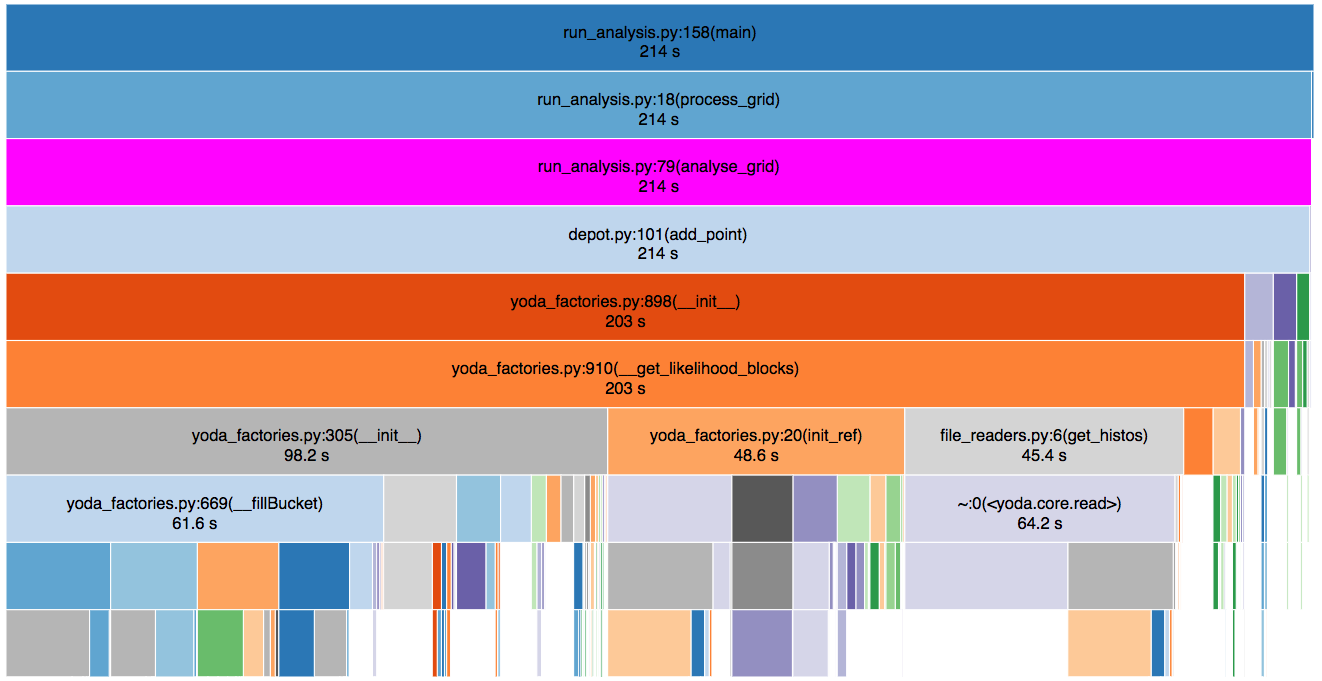
\includegraphics[scale=0.3]{plots/final_grid_profile.png}
\caption{Final Grid Profile}
\label{fig:final_grid_profile}
\end{figure}

\section{Future Work}
